\documentclass[12pt, notitlepage]{article}

\usepackage[letterpaper, margin=1in]{geometry}
\usepackage{graphicx}

\setlength\parindent{0pt}

\title{Interactive comment to ``The Aerosol Limb Imager: acousto-optic imaging of limb scattered
sunlight for stratospheric aerosol profiling'' by B. J. Elash et al}

\author{B.~J. Elash et al. (brenden.elash@usask.ca)}

\begin{document}

\begin{titlepage}
\maketitle
\end{titlepage}


We would like to thank the referee for their helpful comments and suggestions. Below are the referee's comments in italics followed by our reply.

\hrulefill

\textit{Equations should have numbers. Now some of them have random identification numbers.}\\

\textbf{Reply:} Corrected.

\hrulefill

\textit{p. 8, l. 2: Telecentric and telesopic systems. I am not familiar with these terms. Perhaps you could define them briefly.}\\

\textbf{Reply:} Brief descriptions of the terms were added: ``\ldots telecentric and telescopic systems. The telecentric system uses a layout that removes perspective from the image and object plane by creating a condition that requires the chief ray to be parallel to the optical axis in both object and image space. The telescopic system uses a simple two lens afocal system to resize and collimate the incoming rays of light into the AOTF.''

\hrulefill

\textit{Sec. 3.3: Please provide some quantitative estimates of the magnitude of the stray light compared to the signal.}\\

\textbf{Reply:}Using an average of the entire FOV, a stray light to signal ratio of $2.5\cdot10^{-2}$ is noted. A sentence has been added into section 3.3.

\hrulefill

\textit{p.17, l. 16: The value of z\_ref?}\\

\textbf{Reply:} The following sentence has been modified to include the typical values of $z_{ref}$. ``For the ALI measurements, the highest
possible tangent altitude where the signal is above the noise threshold is
approximately 30\,km tangent height and typical values for $z_{ref}$ were between 27 and 30\,km''

\hrulefill

\textit{p.17, l. 16: Perhaps you should differentiate the observed values from the modeled values by improving notation (`m' or `model',\ldots).}\\

\textbf{Reply:} The notation model has been added to the equation.

\hrulefill

\textit{p. 17, l. 28: Is MART better than, for example, Levenberg-Marquatd minimization?
What is the function you minimize by MART? Is it quadratic distance (y\_obsy\_model)**2
or something else?}\\

\textbf{Reply:} The MART method minimizes the function $y_{obs}/y_{mod}*\ln(y_{obs}/y_{mod})$. For application
used here MART and Levenberg-Marquatd return similar results. MART was selected since the OSIRIS aerosol
product uses MART and would help to negate errors from algorithm differences in comparing the results and helps in the intercomparison.

\hrulefill

\textit{Fig. 7: What are the thin horizontal and vertical lines?}\\

\textbf{Reply:} No thin horizontal or vertical lines are noted in the figure produced for the AMTD paper.

\hrulefill

\textit{Fig. 8: Fig. (a) looks very dark.}\\

\textbf{Reply:} Fig. 8 (a) brightness has been increased by 20\% and makes the image easier to read and view. See Figure 1 for the updated figure.

\hrulefill

\textit{Fig. 10. Provide the zenith angle step used to generate the dashed and solid lines.}\\

\textbf{Reply:} For the measurements during the mission a zenith angle step of approximately 2 degrees occurred.
Dashed lines represent solar zenith angles grater than 90 degrees, solid line are profiles with solar zenith angles less than 90.
A sentence in the figure caption has been added to include this information.

\hrulefill

\textit{p.20, l.28: Tack or tackle?}\\

\textbf{Reply:} Corrected.

\hrulefill

\begin{figure}[H]
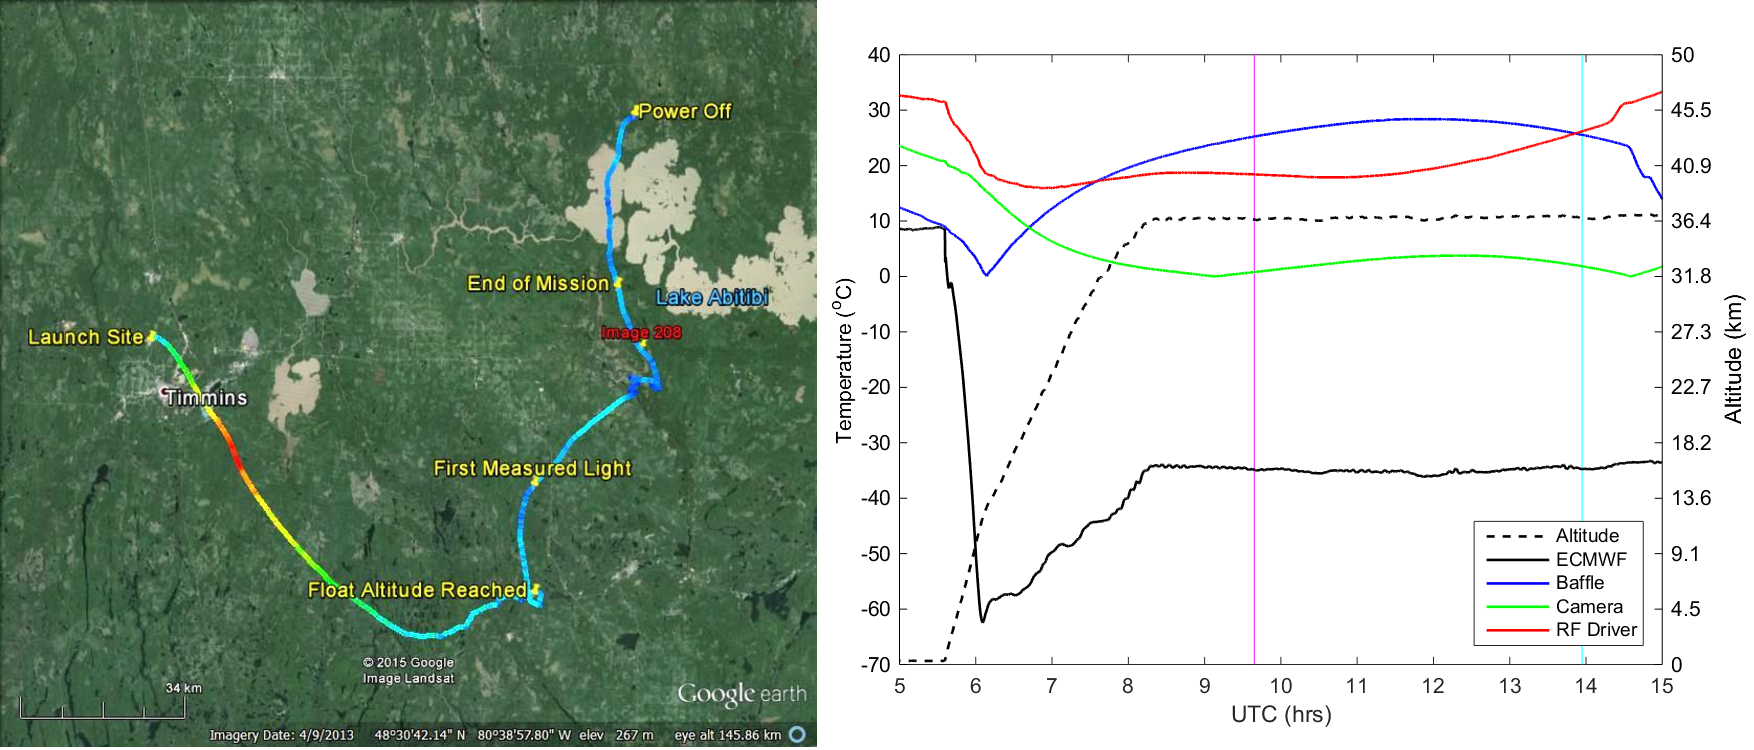
\includegraphics[width=120mm]{amt-2015-329-discussions-f08.pdf}
\caption{\textbf{(a)} The GPS data from ALI during the Nimbus 7
  mission generated via Google Earth. The colour of the line
  represents the absolute speed of the gondola during the
  mission and the blue, green, red colours represent speeds of approximately
  10, 70, and 140~km/h. Important landmarks are noted on the image.  The end of
  mission represent the end of the aerosol mission. No GPS data was
  collected from ALI after power down. The location of image 208 is
  the red label. \textbf{(b)} The temperature and altitude profiles
  from the NIMBUS 7 flight.  The time of image 208 is shown by the
  cyan vertical line and first light measured by ALI is represented by the
  magenta vertical line.}
\label{amtd-2015-0329-f08.pdf}
\end{figure}


\end{document}

